
\subsection{Answers}
\begin{table}[htb]%
\begin{center}%
\caption{Q12: Which MPI implementations do you use?}%
\label{tab:Q12-ans}%
\begin{tabular}{l|l|r}%
\hline%
Choice & Abbrv. & \# Answers \\%
\hline%
Open MPI & OMPI & 723 (85.4\%) \\%
Intel MPI & Intel & 522 (61.6\%) \\%
MPICH & MPICH & 470 (55.5\%) \\%
MVAPICH & MVA & 175 (20.7\%) \\%
Cray MPI & Cray & 145 (17.1\%) \\%
IBM MPI (BG/Q, PE, Spectrum) & IBM & 92 (10.9\%) \\%
Fujistu MPI & Fujitsu & 29 (3.4\%) \\%
MS MPI & MS & 27 (3.2\%) \\%
HPE MPI & HPE & 23 (2.7\%) \\%
NEC MPI & NEC & 23 (2.7\%) \\%
I do not know & No idea & 10 (1.2\%) \\%
MPC MPI & MPC & 8 (0.9\%) \\%
Sunway MPI & Sunway & 5 (0.6\%) \\%
Tianhe MPI & Tianhe & 3 (0.4\%) \\%
other & - & 27 (3.2\%) \\%
\hline%
\multicolumn{2}{c}{total} & 2282 (847)\\%
\hline%
\end{tabular}%
\end{center}%
\end{table}%


\begin{figure}[htb]
\begin{center}
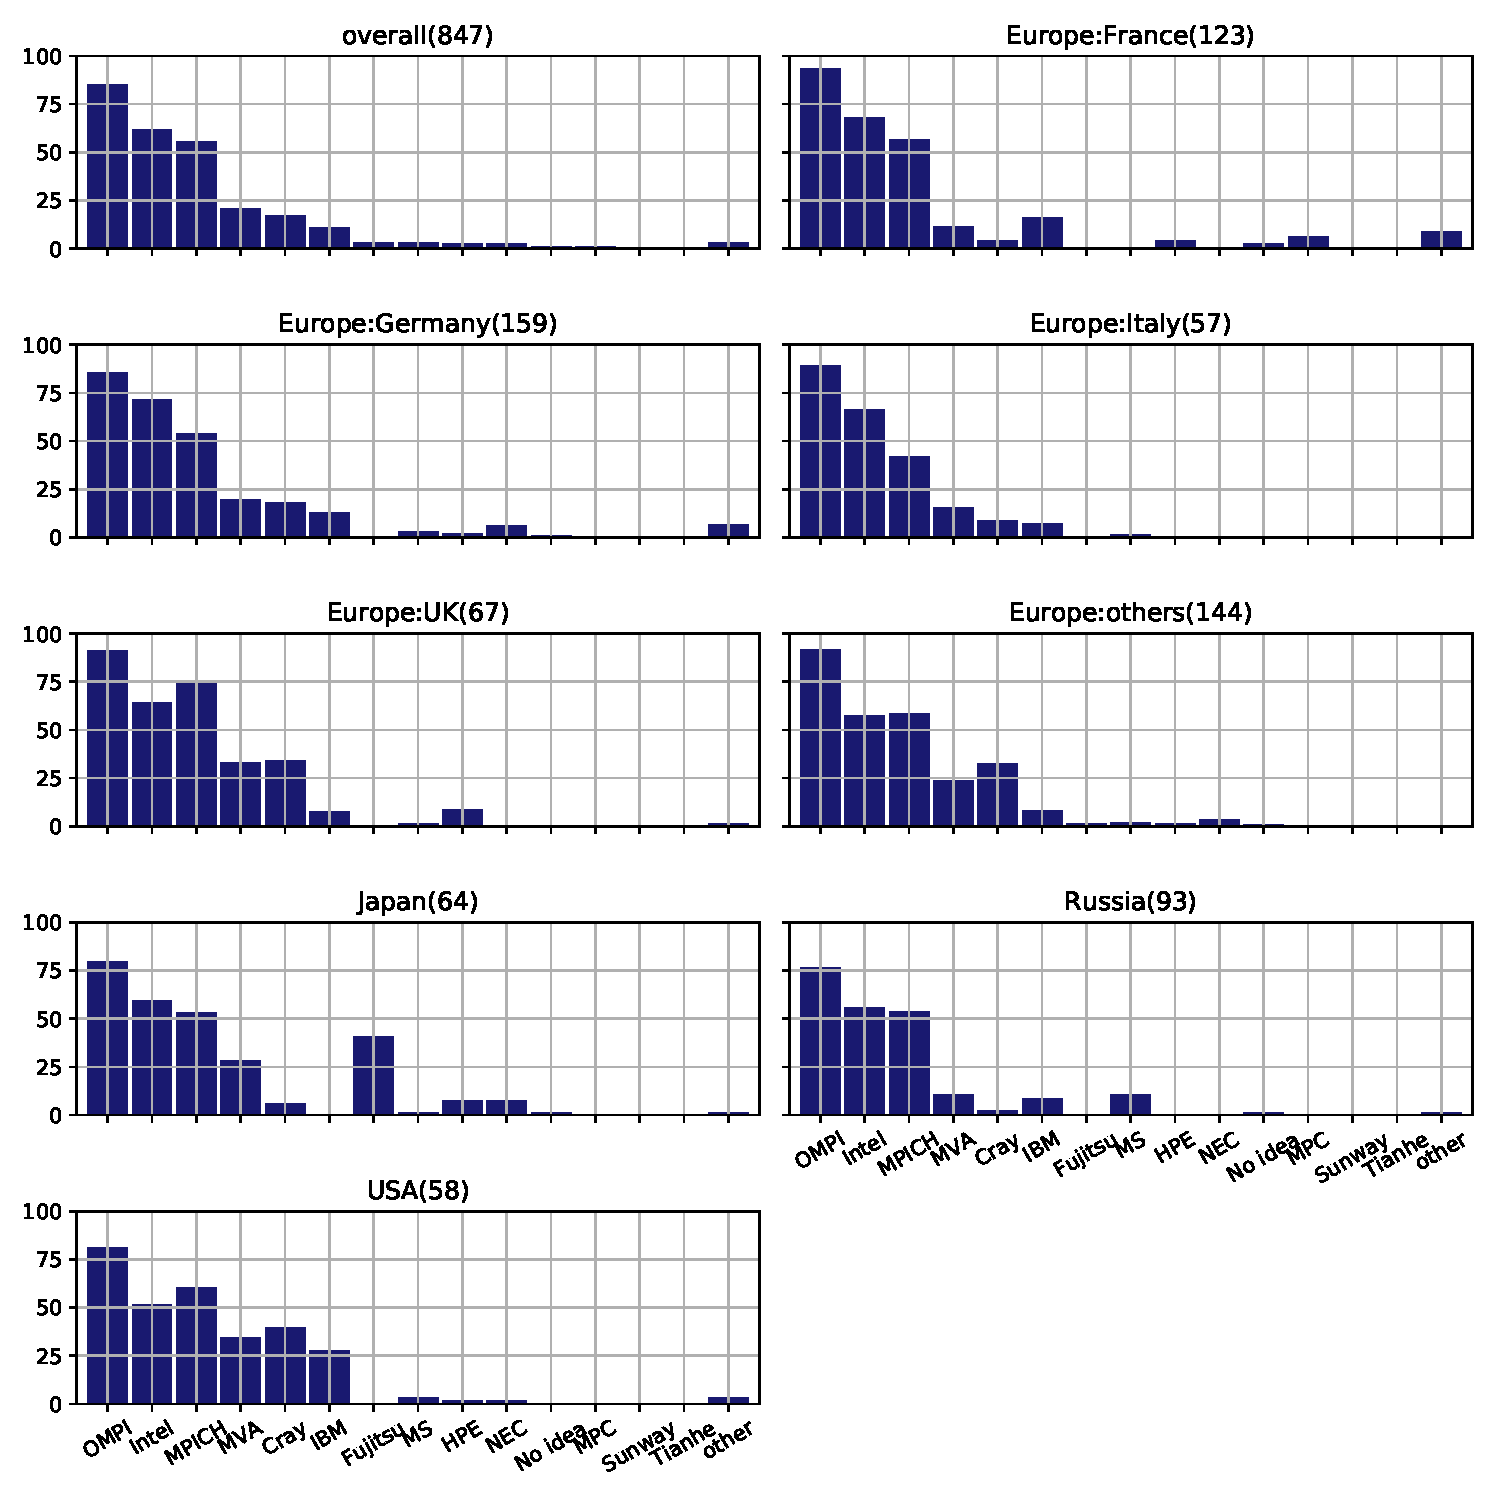
\includegraphics[width=10cm]{../pdfs/Q12.pdf}
\caption{Breakdown of MPI implementation usages per location}
\label{fig:Q12}
\end{center}
\end{figure}

\begin{figure}[htb]
\begin{center}
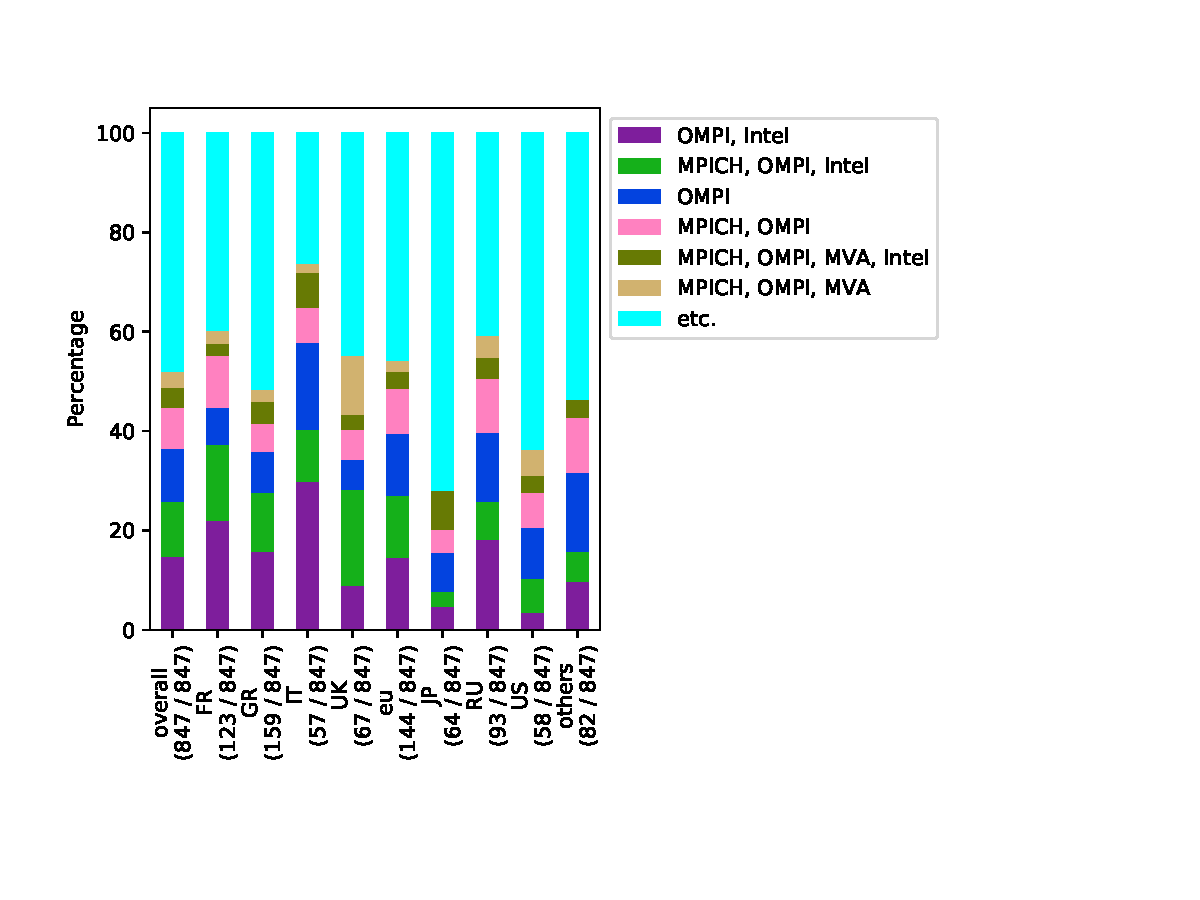
\includegraphics[width=14cm]{../pdfs/Q12-mans.pdf}
\caption{Multiple Answer: Q12}
\label{fig:Q12-mans}
\end{center}
\end{figure}

Looking more precisely at the 27 other MPI implementations specifically
mentioned in the answers, points to the expected dichotomy of vendor's imposed
or delivered MPI implementations, as well as to some lesser known MPI
implementations with an existing, but usually geographically constrained user
base, such as MadMPI with 4 mentions only in Europe:France and ParaStation~MPI
with 10 mentions only in Europe:Germany. Out of them only one MPI implementation
stands out with a more international user base, SGI MPI with 5 total mentions,
all across the world. Finally, for the sake of completeness it should be noted
that some MPI implementations were mentioned at least once (Sun~MPI,
Adaptive~MPI, PGI~MPI, Platform~MPI) as well as a Python API for MPI (mpi4py).

% \mycomment[AH]{I do not think they are geographically constrained, but
% vendors force users to use their MPI. For example, BG/* users have no
% choice but using IBM MPI, the K users must use Fujistu MPI.}.

% \mycomment[AH]{It would be nice to categorize MPI implementations into
% two; proprietary (vendor) MPI and public domain MPI}.

Looking at this list from the perspective of the origin of the MPI
implementation, either public domain or proprietary (vendor) provided MPI we can
notice that about 60\% of the answers are using open source MPI
implementations (Open MPI, MPICH and MVAPICH)  not provided by a
vendor. 

In all countries and regions, Open MPI, Inel MPI and MPICH dominate
more than 60\%. Intel MPI is the most widely used vendor provided MPI
implementation. Cray MPI dominates around 10\% in most countries and
regions though, Fujistu MPI dominates more than Cray MPI in Japan.

In Table~\ref{tab:Q12-mans}, Open MPI is the most frequently used MPI
implementation in the standalone way.  Although the K computer and its
successors only support Fujitsu MPI, most machines support several
MPI implementations. It would be interesting to know how users choose
an MPI implementation among them.

\clearpage%
{\footnotesize\begin{landscape}%
\begin{longtable}[htb]{r|c|c|c|c|c|c|c|c|c|c}%
\caption{Q12: Which MPI implementations do you use?}%
\label{tab:Q12-mans} \\%
\hline%
Multi-Answer & overall & FR & GR & IT & UK & eu & JP & RU & US & others \\
 \hline%
\endfirsthead%
\multicolumn{11}{r}{(continued from the previous page)}\\%
\hline%
Multi-Answer & overall & FR & GR & IT & UK & eu & JP & RU & US & others \\
 \hline%
\endhead%
\hline%
(total) & 847 & 123 & 159 & 57 & 67 & 144 & 64 & 93 & 58 & 82 \\%
\hline%
\multicolumn{11}{r}{(continue to the next page)}\\%
\endfoot%
\hline%
(total) & 847 & 123 & 159 & 57 & 67 & 144 & 64 & 93 & 58 & 82 \\%
\hline%
\endlastfoot%
\hline%
{OMPI, Intel} & 126 & 27 & 25 & 17 & 6 & 21 & 3 & 17 & 2 & 8 \\%
{MPICH, OMPI, Intel} & 93 & 19 & 19 & 6 & 13 & 18 & 2 & 7 & 4 & 5 \\%
{OMPI} & 91 & 9 & 13 & 10 & 4 & 18 & 5 & 13 & 6 & 13 \\%
{MPICH, OMPI} & 69 & 13 & 9 & 4 & 4 & 13 & 3 & 10 & 4 & 9 \\%
{MPICH, OMPI, MVA, Intel} & 35 & 3 & 7 & 4 & 2 & 5 & 5 & 4 & 2 & 3 \\%
{MPICH, OMPI, MVA} & 26 & 3 & 4 & 1 & 8 & 3 & 0 & 4 & 3 & 0 \\%
{Intel} & 23 & 2 & 6 & 2 & 0 & 3 & 0 & 6 & 1 & 3 \\%
{MPICH, Intel} & 20 & 1 & 3 & 2 & 1 & 1 & 2 & 7 & 0 & 3 \\%
{OMPI, MVA, Intel} & 19 & 2 & 2 & 1 & 2 & 3 & 2 & 0 & 2 & 5 \\%
{MPICH} & 18 & 1 & 3 & 1 & 1 & 1 & 1 & 4 & 1 & 5 \\%
{MPICH, OMPI, Intel, Cray} & 18 & 1 & 4 & 0 & 3 & 5 & 1 & 0 & 4 & 0 \\%
{MPICH, OMPI, Intel, IBM} & 16 & 6 & 5 & 1 & 0 & 2 & 0 & 2 & 0 & 0 \\%
{OMPI, Intel, Cray} & 14 & 0 & 4 & 2 & 3 & 3 & 0 & 0 & 2 & 0 \\%
{MPICH, OMPI, MVA, Intel, Cray} & 14 & 0 & 2 & 0 & 4 & 4 & 1 & 0 & 3 & 0 \\%
{MPICH, OMPI, Cray} & 14 & 0 & 3 & 1 & 1 & 9 & 0 & 0 & 0 & 0 \\%
{MPICH, OMPI, Intel, Cray, IBM} & 10 & 1 & 2 & 0 & 0 & 3 & 0 & 0 & 2 & 2 \\%
{No idea} & 9 & 3 & 1 & 0 & 0 & 1 & 1 & 1 & 0 & 2 \\%
{MPICH, OMPI, MVA, Cray} & 8 & 0 & 1 & 0 & 1 & 6 & 0 & 0 & 0 & 0 \\%
{MPICH, OMPI, MVA, Intel, IBM} & 7 & 2 & 3 & 0 & 0 & 1 & 0 & 1 & 0 & 0 \\%
{OMPI, IBM} & 7 & 2 & 0 & 0 & 0 & 0 & 0 & 2 & 3 & 0 \\%
{OMPI, Cray} & 7 & 0 & 3 & 0 & 0 & 2 & 0 & 0 & 0 & 2 \\%
{MPICH, OMPI, MVA, Intel, Cray, IBM} & 7 & 1 & 1 & 2 & 1 & 0 & 0 & 0 & 1 & 1 \\%
{MPICH, OMPI, Intel, Fujitsu} & 6 & 0 & 1 & 0 & 0 & 0 & 5 & 0 & 0 & 0 \\%
{MPICH, OMPI, Intel, MS} & 6 & 1 & 3 & 0 & 0 & 0 & 0 & 2 & 0 & 0 \\%
{MVA} & 6 & 0 & 0 & 0 & 0 & 0 & 3 & 0 & 1 & 2 \\%
{OMPI, Intel, IBM} & 5 & 1 & 0 & 0 & 1 & 1 & 0 & 0 & 0 & 2 \\%
{OMPI, Intel, HPE} & 5 & 1 & 1 & 0 & 0 & 1 & 2 & 0 & 0 & 0 \\%
{MPICH, OMPI, IBM} & 5 & 0 & 2 & 1 & 0 & 0 & 0 & 1 & 1 & 0 \\%
{OMPI, Intel, MS} & 5 & 0 & 1 & 0 & 0 & 0 & 0 & 3 & 0 & 1 \\%
{MPICH, Cray} & 5 & 0 & 0 & 0 & 3 & 1 & 0 & 0 & 1 & 0 \\%
{MPICH, OMPI, MS} & 4 & 0 & 0 & 0 & 1 & 0 & 1 & 2 & 0 & 0 \\%
{MPICH, OMPI, Intel, Cray, NEC} & 4 & 0 & 2 & 0 & 0 & 2 & 0 & 0 & 0 & 0 \\%
{MPICH, OMPI, Intel, HPE} & 4 & 1 & 1 & 0 & 1 & 0 & 1 & 0 & 0 & 0 \\%
{ParaStation MPI} & 4 & 0 & 4 & 0 & 0 & 0 & 0 & 0 & 0 & 0 \\%
{MPICH, OMPI, Cray, IBM} & 4 & 0 & 0 & 0 & 1 & 0 & 0 & 0 & 2 & 1 \\%
{MPICH, MS} & 3 & 0 & 0 & 0 & 0 & 0 & 0 & 2 & 0 & 1 \\%
{OMPI, Intel, Fujitsu} & 3 & 0 & 0 & 0 & 0 & 0 & 3 & 0 & 0 & 0 \\%
{MPICH, MVA, Intel} & 3 & 0 & 0 & 1 & 0 & 0 & 0 & 0 & 0 & 2 \\%
{MPICH, OMPI, Fujitsu} & 3 & 0 & 0 & 0 & 0 & 0 & 3 & 0 & 0 & 0 \\%
{MPICH, OMPI, MVA, Intel, Cray, HPE} & 3 & 0 & 0 & 0 & 3 & 0 & 0 & 0 & 0 & 0 \\%
{MPICH, OMPI, Fujitsu, NEC} & 3 & 0 & 0 & 0 & 0 & 0 & 3 & 0 & 0 & 0 \\%
{MPICH, MVA} & 3 & 0 & 0 & 0 & 0 & 1 & 0 & 0 & 1 & 1 \\%
{MPICH, MVA, Cray} & 3 & 0 & 0 & 0 & 0 & 2 & 0 & 0 & 1 & 0 \\%
{OMPI, MVA} & 3 & 0 & 1 & 0 & 0 & 0 & 0 & 1 & 0 & 1 \\%
{MPICH, OMPI, Intel, NEC} & 3 & 0 & 1 & 0 & 0 & 1 & 1 & 0 & 0 & 0 \\%
{OMPI, Intel, Cray, IBM} & 2 & 1 & 0 & 0 & 0 & 1 & 0 & 0 & 0 & 0 \\%
{OMPI, HPE} & 2 & 1 & 0 & 0 & 0 & 0 & 0 & 0 & 0 & 1 \\%
{MPICH, OMPI, MVA, Intel, Cray, IBM, HPE} & 2 & 1 & 0 & 0 & 1 & 0 & 0 & 0 & 0 & 0 \\%
{MPICH, OMPI, MPC} & 2 & 2 & 0 & 0 & 0 & 0 & 0 & 0 & 0 & 0 \\%
{OMPI, MVA, Cray} & 2 & 0 & 0 & 0 & 0 & 2 & 0 & 0 & 0 & 0 \\%
{MPICH, MVA, Intel, Cray} & 2 & 0 & 0 & 0 & 0 & 1 & 0 & 0 & 1 & 0 \\%
{Intel, Fujitsu} & 2 & 0 & 0 & 0 & 0 & 0 & 2 & 0 & 0 & 0 \\%
{OMPI, MVA, Intel, IBM} & 2 & 0 & 1 & 0 & 0 & 1 & 0 & 0 & 0 & 0 \\%
{OMPI, Intel, IBM, HPE} & 2 & 1 & 1 & 0 & 0 & 0 & 0 & 0 & 0 & 0 \\%
{MPICH, OMPI, MVA, Fujitsu} & 2 & 0 & 0 & 0 & 0 & 0 & 2 & 0 & 0 & 0 \\%
{Intel, IBM} & 2 & 0 & 1 & 0 & 0 & 1 & 0 & 0 & 0 & 0 \\%
{MPICH, Intel, IBM} & 2 & 1 & 1 & 0 & 0 & 0 & 0 & 0 & 0 & 0 \\%
{MPICH, OMPI, MVA, Intel, Cray, NEC} & 2 & 0 & 1 & 0 & 0 & 0 & 0 & 0 & 0 & 1 \\%
{OMPI, MVA, Intel, Fujitsu} & 2 & 0 & 0 & 0 & 0 & 0 & 2 & 0 & 0 & 0 \\%
{Intel, Cray} & 2 & 0 & 0 & 0 & 0 & 0 & 2 & 0 & 0 & 0 \\%
{MPICH, OMPI, MVA, Intel, Fujitsu} & 2 & 0 & 0 & 0 & 0 & 0 & 2 & 0 & 0 & 0 \\%
{OMPI, Fujitsu} & 2 & 0 & 0 & 0 & 0 & 0 & 2 & 0 & 0 & 0 \\%
{MPICH, Intel, Cray} & 1 & 0 & 0 & 0 & 0 & 0 & 0 & 1 & 0 & 0 \\%
{MVA, Intel} & 1 & 0 & 0 & 0 & 0 & 0 & 0 & 0 & 1 & 0 \\%
{MPICH, OMPI, Intel, Tianhe, Sunway} & 1 & 0 & 0 & 0 & 0 & 0 & 0 & 0 & 0 & 1 \\%
{OMPI, Intel, Cray, NEC} & 1 & 0 & 1 & 0 & 0 & 0 & 0 & 0 & 0 & 0 \\%
{MPICH, OMPI, MVA, Intel, IBM, ParaStation MPI} & 1 & 0 & 1 & 0 & 0 & 0 & 0 & 0 & 0 & 0 \\%
{MPICH, OMPI, Intel, Cray, SGI MPI} & 1 & 0 & 0 & 0 & 0 & 0 & 0 & 1 & 0 & 0 \\%
{MPICH, OMPI, Cray, MS} & 1 & 0 & 0 & 0 & 0 & 1 & 0 & 0 & 0 & 0 \\%
{MPICH, OMPI, MVA, IBM} & 1 & 0 & 0 & 0 & 0 & 0 & 0 & 0 & 1 & 0 \\%
{OMPI, MVA, Intel, Cray, NEC} & 1 & 0 & 1 & 0 & 0 & 0 & 0 & 0 & 0 & 0 \\%
{Fujitsu} & 1 & 0 & 0 & 0 & 0 & 0 & 1 & 0 & 0 & 0 \\%
{OMPI, Intel, Cray, IBM, HPE} & 1 & 0 & 0 & 0 & 1 & 0 & 0 & 0 & 0 & 0 \\%
{MPICH, OMPI, Intel, IBM, SGI MPI} & 1 & 1 & 0 & 0 & 0 & 0 & 0 & 0 & 0 & 0 \\%
{OMPI, Intel, Cray, IBM, MS} & 1 & 0 & 0 & 0 & 0 & 0 & 0 & 0 & 1 & 0 \\%
{OMPI, Intel, MPC} & 1 & 1 & 0 & 0 & 0 & 0 & 0 & 0 & 0 & 0 \\%
{MPICH, OMPI, HPE} & 1 & 0 & 0 & 0 & 0 & 0 & 1 & 0 & 0 & 0 \\%
{MPICH, Intel, Cray, SGI MPT} & 1 & 0 & 0 & 0 & 1 & 0 & 0 & 0 & 0 & 0 \\%
{MS} & 1 & 0 & 0 & 0 & 0 & 0 & 0 & 0 & 0 & 1 \\%
{OMPI, MVA, Intel, HPE} & 1 & 0 & 0 & 0 & 0 & 0 & 1 & 0 & 0 & 0 \\%
{MPICH, OMPI, Intel, Tianhe} & 1 & 0 & 0 & 0 & 0 & 0 & 0 & 0 & 0 & 1 \\%
{MPICH, OMPI, MVA, Intel, Cray, IBM, Fujitsu} & 1 & 0 & 0 & 0 & 0 & 1 & 0 & 0 & 0 & 0 \\%
{OMPI, MPC} & 1 & 1 & 0 & 0 & 0 & 0 & 0 & 0 & 0 & 0 \\%
{MPICH, OMPI, Intel, BULL MPI} & 1 & 1 & 0 & 0 & 0 & 0 & 0 & 0 & 0 & 0 \\%
{OMPI, Intel, IBM, NEC} & 1 & 0 & 1 & 0 & 0 & 0 & 0 & 0 & 0 & 0 \\%
{Intel, Cray, IBM} & 1 & 0 & 1 & 0 & 0 & 0 & 0 & 0 & 0 & 0 \\%
{OMPI, MVA, Intel, NEC} & 1 & 0 & 1 & 0 & 0 & 0 & 0 & 0 & 0 & 0 \\%
{MPICH, OMPI, MadMPI} & 1 & 1 & 0 & 0 & 0 & 0 & 0 & 0 & 0 & 0 \\%
{MPICH, OMPI, MVA, Intel, Cray, MS} & 1 & 0 & 0 & 0 & 0 & 1 & 0 & 0 & 0 & 0 \\%
{MPICH, OMPI, Intel, ParaStation MPI} & 1 & 0 & 1 & 0 & 0 & 0 & 0 & 0 & 0 & 0 \\%
{MPICH, OMPI, MVA, Intel, Cray, IBM, NEC} & 1 & 0 & 1 & 0 & 0 & 0 & 0 & 0 & 0 & 0 \\%
{MPICH, OMPI, BullMPI} & 1 & 1 & 0 & 0 & 0 & 0 & 0 & 0 & 0 & 0 \\%
{MPICH, OMPI, MVA, Cray, MS} & 1 & 0 & 0 & 0 & 0 & 1 & 0 & 0 & 0 & 0 \\%
{MPICH, OMPI, No idea} & 1 & 0 & 1 & 0 & 0 & 0 & 0 & 0 & 0 & 0 \\%
{MPICH, OMPI, MVA, Intel, MPC} & 1 & 1 & 0 & 0 & 0 & 0 & 0 & 0 & 0 & 0 \\%
{Sunway} & 1 & 0 & 0 & 0 & 0 & 0 & 0 & 0 & 0 & 1 \\%
{OMPI, MVA, Intel, Cray, IBM} & 1 & 0 & 0 & 0 & 0 & 1 & 0 & 0 & 0 & 0 \\%
{OMPI, Intel, MPC, madMPI} & 1 & 1 & 0 & 0 & 0 & 0 & 0 & 0 & 0 & 0 \\%
{MPICH, MVA, Cray, IBM} & 1 & 0 & 0 & 0 & 0 & 0 & 0 & 0 & 1 & 0 \\%
{MPICH, OMPI, MVA, Intel, MPC, MadMPI} & 1 & 1 & 0 & 0 & 0 & 0 & 0 & 0 & 0 & 0 \\%
{MPICH, OMPI, Intel, IBM, BullX-MPI} & 1 & 1 & 0 & 0 & 0 & 0 & 0 & 0 & 0 & 0 \\%
{MPICH, OMPI, MVA, Intel, ParaStation MPI} & 1 & 0 & 1 & 0 & 0 & 0 & 0 & 0 & 0 & 0 \\%
{Intel, ParaStation MPI} & 1 & 0 & 1 & 0 & 0 & 0 & 0 & 0 & 0 & 0 \\%
{Intel, Fujitsu, NEC, SGI MPI} & 1 & 0 & 0 & 0 & 0 & 0 & 1 & 0 & 0 & 0 \\%
{MPICH, Intel, Sunway} & 1 & 0 & 0 & 0 & 0 & 0 & 0 & 0 & 0 & 1 \\%
{Intel, MS} & 1 & 0 & 1 & 0 & 0 & 0 & 0 & 0 & 0 & 0 \\%
{MPICH, OMPI, Intel, IBM, MS} & 1 & 0 & 0 & 0 & 0 & 0 & 0 & 1 & 0 & 0 \\%
{MPICH, OMPI, NEC} & 1 & 1 & 0 & 0 & 0 & 0 & 0 & 0 & 0 & 0 \\%
{OMPI, MVA, Intel, Cray} & 1 & 0 & 1 & 0 & 0 & 0 & 0 & 0 & 0 & 0 \\%
{OMPI, Intel, Tianhe} & 1 & 0 & 0 & 0 & 0 & 0 & 0 & 0 & 0 & 1 \\%
{MPICH, OMPI, mpi4py} & 1 & 1 & 0 & 0 & 0 & 0 & 0 & 0 & 0 & 0 \\%
{OMPI, Cray, NEC} & 1 & 0 & 0 & 0 & 0 & 0 & 0 & 0 & 1 & 0 \\%
{MPICH, OMPI, Intel, madmpi} & 1 & 1 & 0 & 0 & 0 & 0 & 0 & 0 & 0 & 0 \\%
{MPICH, OMPI, MVA, Intel, Cray, Fujitsu, NEC} & 1 & 0 & 0 & 0 & 0 & 1 & 0 & 0 & 0 & 0 \\%
{OMPI, Intel, HPE, NEC} & 1 & 0 & 0 & 0 & 0 & 1 & 0 & 0 & 0 & 0 \\%
{MVA, Sunway} & 1 & 0 & 0 & 0 & 0 & 0 & 0 & 0 & 0 & 1 \\%
{OMPI, Intel, ParaStation MPI} & 1 & 0 & 1 & 0 & 0 & 0 & 0 & 0 & 0 & 0 \\%
{MPICH, IBM} & 1 & 0 & 0 & 0 & 0 & 0 & 0 & 1 & 0 & 0 \\%
{MVA, Intel, Cray, IBM} & 1 & 0 & 0 & 0 & 0 & 0 & 0 & 0 & 1 & 0 \\%
{MPICH, MVA, Intel, ParaStation MPI} & 1 & 0 & 1 & 0 & 0 & 0 & 0 & 0 & 0 & 0 \\%
{MPICH, OMPI, Intel, IBM, PGI MPI} & 1 & 0 & 0 & 0 & 0 & 0 & 0 & 0 & 1 & 0 \\%
{MPICH, OMPI, Intel, Cray, Sun MPI} & 1 & 0 & 1 & 0 & 0 & 0 & 0 & 0 & 0 & 0 \\%
{OMPI, Cray, IBM} & 1 & 0 & 0 & 0 & 0 & 0 & 0 & 0 & 1 & 0 \\%
{Intel, HPE} & 1 & 0 & 0 & 0 & 0 & 0 & 0 & 0 & 1 & 0 \\%
{OMPI, Sunway} & 1 & 0 & 0 & 0 & 0 & 0 & 0 & 0 & 0 & 1 \\%
{MPICH, OMPI, MVA, Intel, Cray, IBM, MS, Adaptive MPI} & 1 & 0 & 0 & 0 & 0 & 0 & 0 & 0 & 1 & 0 \\%
{MPICH, OMPI, Intel, IBM, BULLMPI} & 1 & 1 & 0 & 0 & 0 & 0 & 0 & 0 & 0 & 0 \\%
{OMPI, MS} & 1 & 0 & 0 & 1 & 0 & 0 & 0 & 0 & 0 & 0 \\%
{MPICH, OMPI, Intel, MPC} & 1 & 1 & 0 & 0 & 0 & 0 & 0 & 0 & 0 & 0 \\%
{MPICH, OMPI, MVA, Intel, NEC} & 1 & 0 & 1 & 0 & 0 & 0 & 0 & 0 & 0 & 0 \\%
{MPICH, OMPI, Intel, Platform} & 1 & 1 & 0 & 0 & 0 & 0 & 0 & 0 & 0 & 0 \\%
\hline%
\end{longtable}%
\end{landscape}}%
\clearpage%


\subsection{List of other answers}

\begin{report}
\begin{itemize}
\item Europe:France: BULL MPI
\item Europe:France: BULLMPI
\item Europe:France: BullMPI
\item Europe:France: BullX-MPI
\item Europe:France: MadMPI
\item Europe:France: MadMPI
\item Europe:France: Platform
\item Europe:France: SGI MPI
\item Europe:France: madMPI
\item Europe:France: madmpi
\item Europe:France: mpi4py
\item Europe:Germany: ParaStation MPI
\item Europe:Germany: ParaStation MPI
\item Europe:Germany: ParaStation MPI
\item Europe:Germany: ParaStation MPI
\item Europe:Germany: ParaStation MPI
\item Europe:Germany: ParaStation MPI
\item Europe:Germany: ParaStation MPI
\item Europe:Germany: ParaStation MPI
\item Europe:Germany: ParaStation MPI
\item Europe:Germany: ParaStation MPI
\item Europe:Germany: Sun MPI
\item Europe:UK: SGI MPT
\item Japan: SGI MPI
\item Russia: SGI MPI
\item USA: Adaptive MPI
\item USA: PGI MPI

\end{itemize}
\end{report}
